Los archivos relacionados a la documentación del proyecto Voorspelling se encuentra en la carpeta \textit{Documentation} del repositorio del proyecto, la cual puede ser consultado en GitHub con el siguiente enlace: \url{https://github.com/Noczio/VoorSpelling}.

Cada carpeta contiene archivos clasificados por su tipo, ya sean diagramas, formatos, flujo de la aplicación, \textit{mockups}, \textit{sketchs} y otros recursos como el cronograma del proyecto. No obstante, los documentos que se presentan a continuación son aquellos relacionados con los requerimientos, \textit{back-end}, \textit{front-end}, casos de uso y pruebas de software desarrolladas durante el ciclo de vida del proyecto desde Agosto del 2020 hasta Marzo del 2021.

%requerimientos
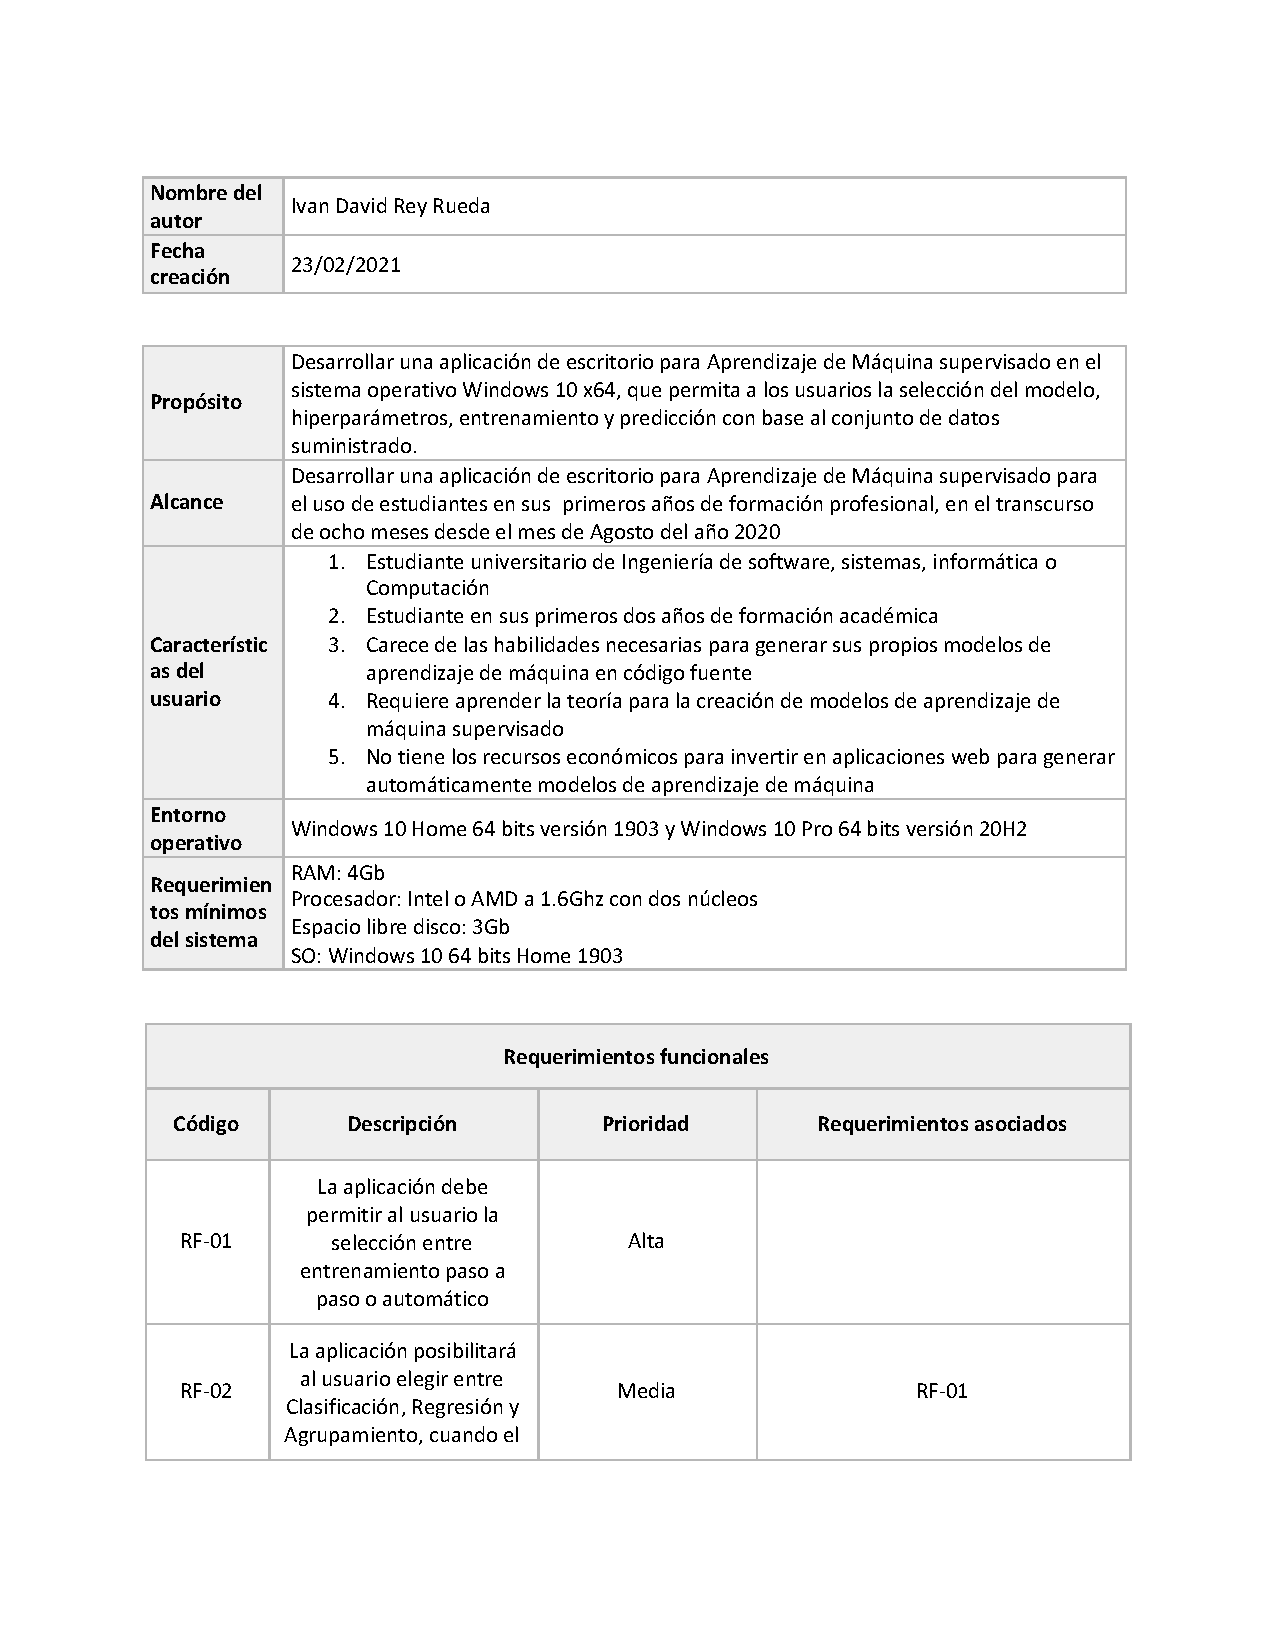
\includepdf[pages=-, pagecommand=\thispagestyle{otherplain} ,width=\textwidth]{pdfs/Requerimientos_proyecto_Firmado.pdf}


%front y back end
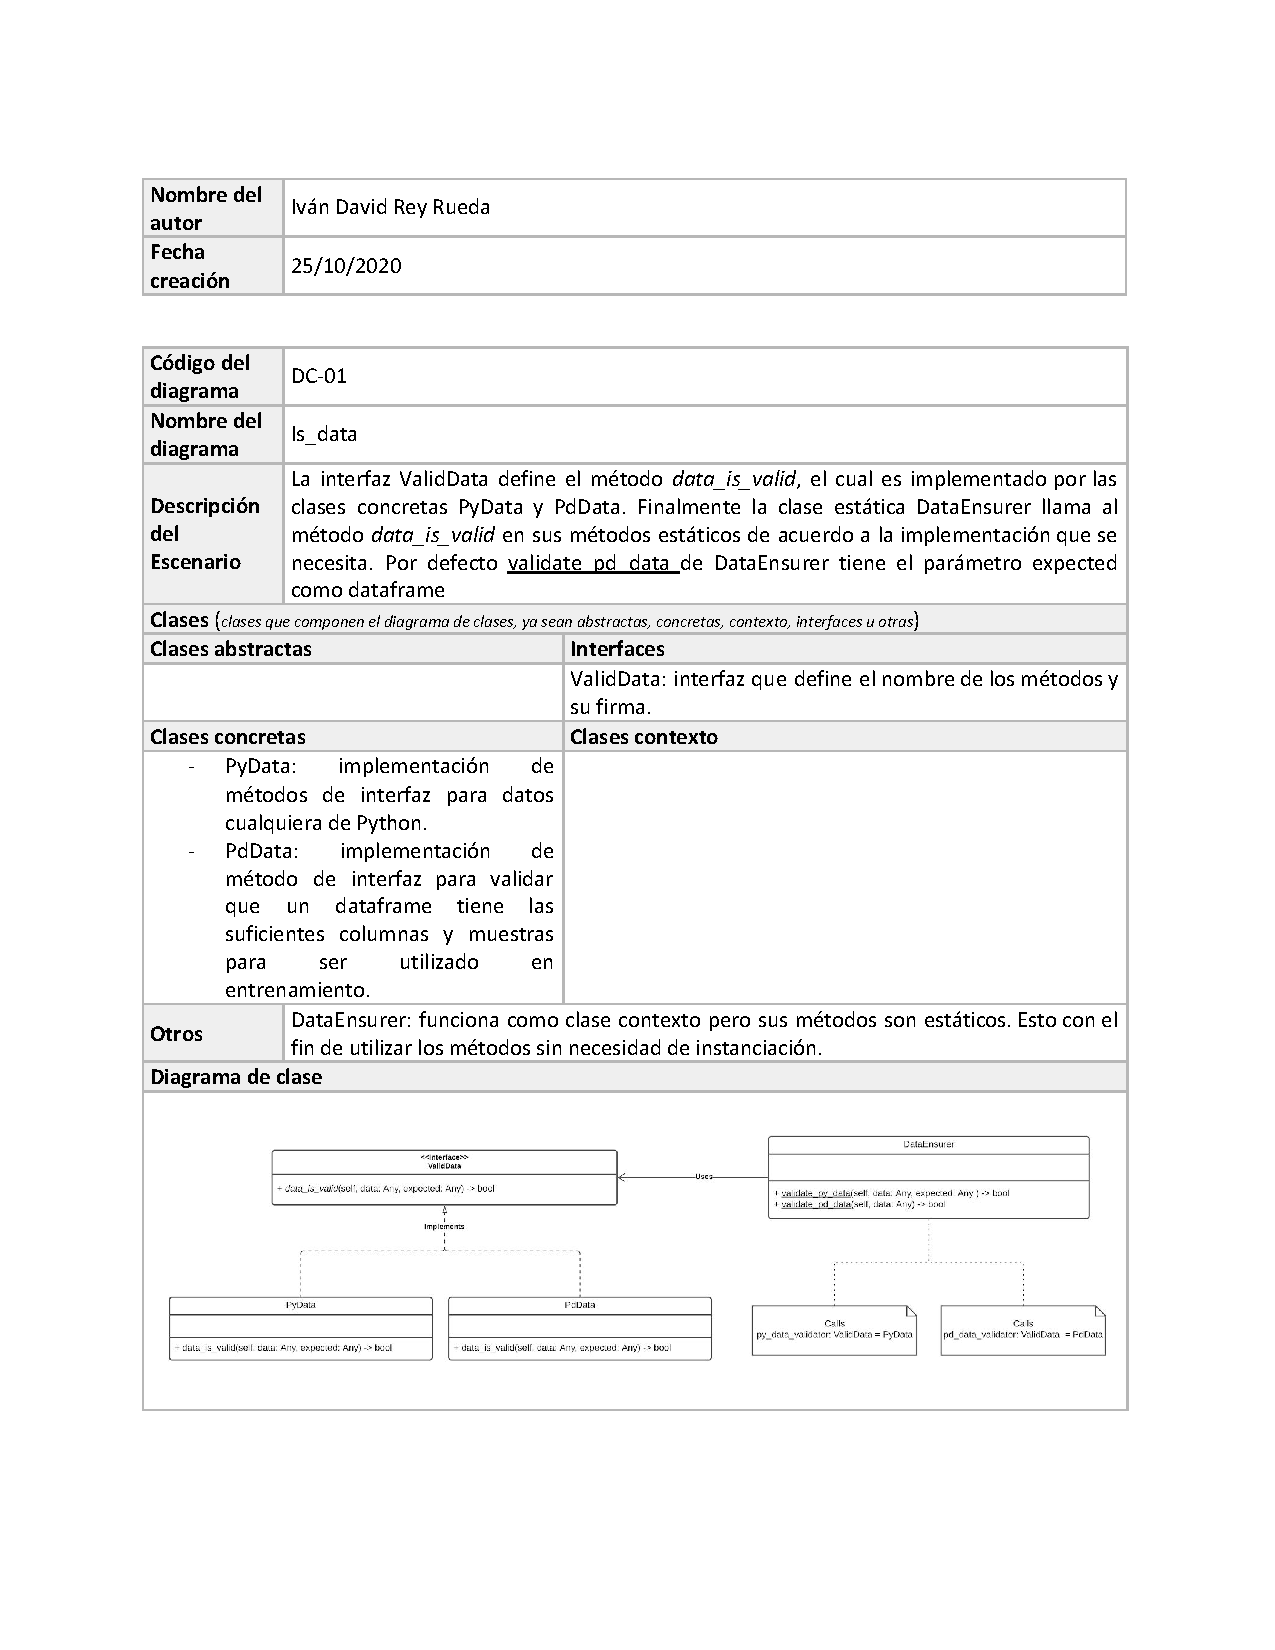
\includepdf[pages=-, pagecommand=\thispagestyle{otherplain} ,width=\textwidth]{pdfs/Formato diagrama de clase DC-01_Firmado.pdf}
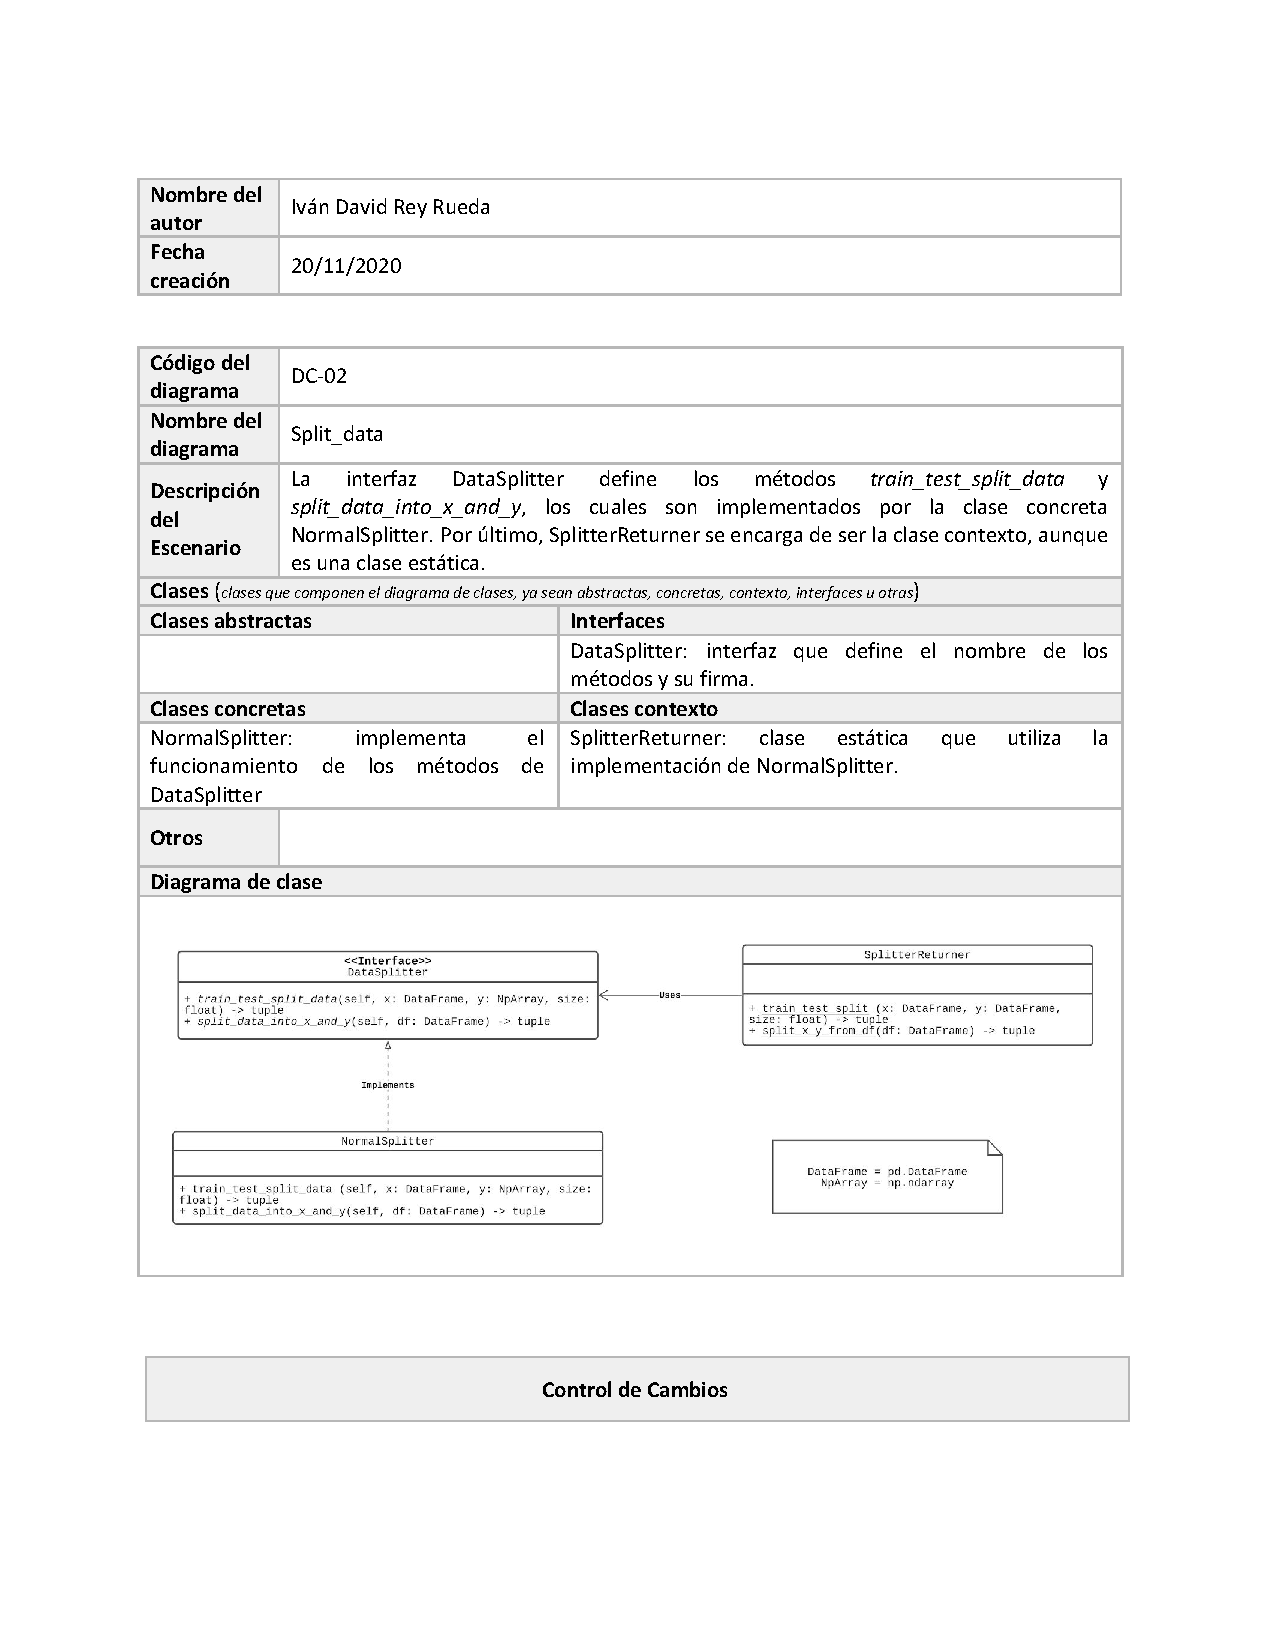
\includepdf[pages=-, pagecommand=\thispagestyle{otherplain}, width=\textwidth]{pdfs/Formato diagrama de clase DC-02_Firmado.pdf}
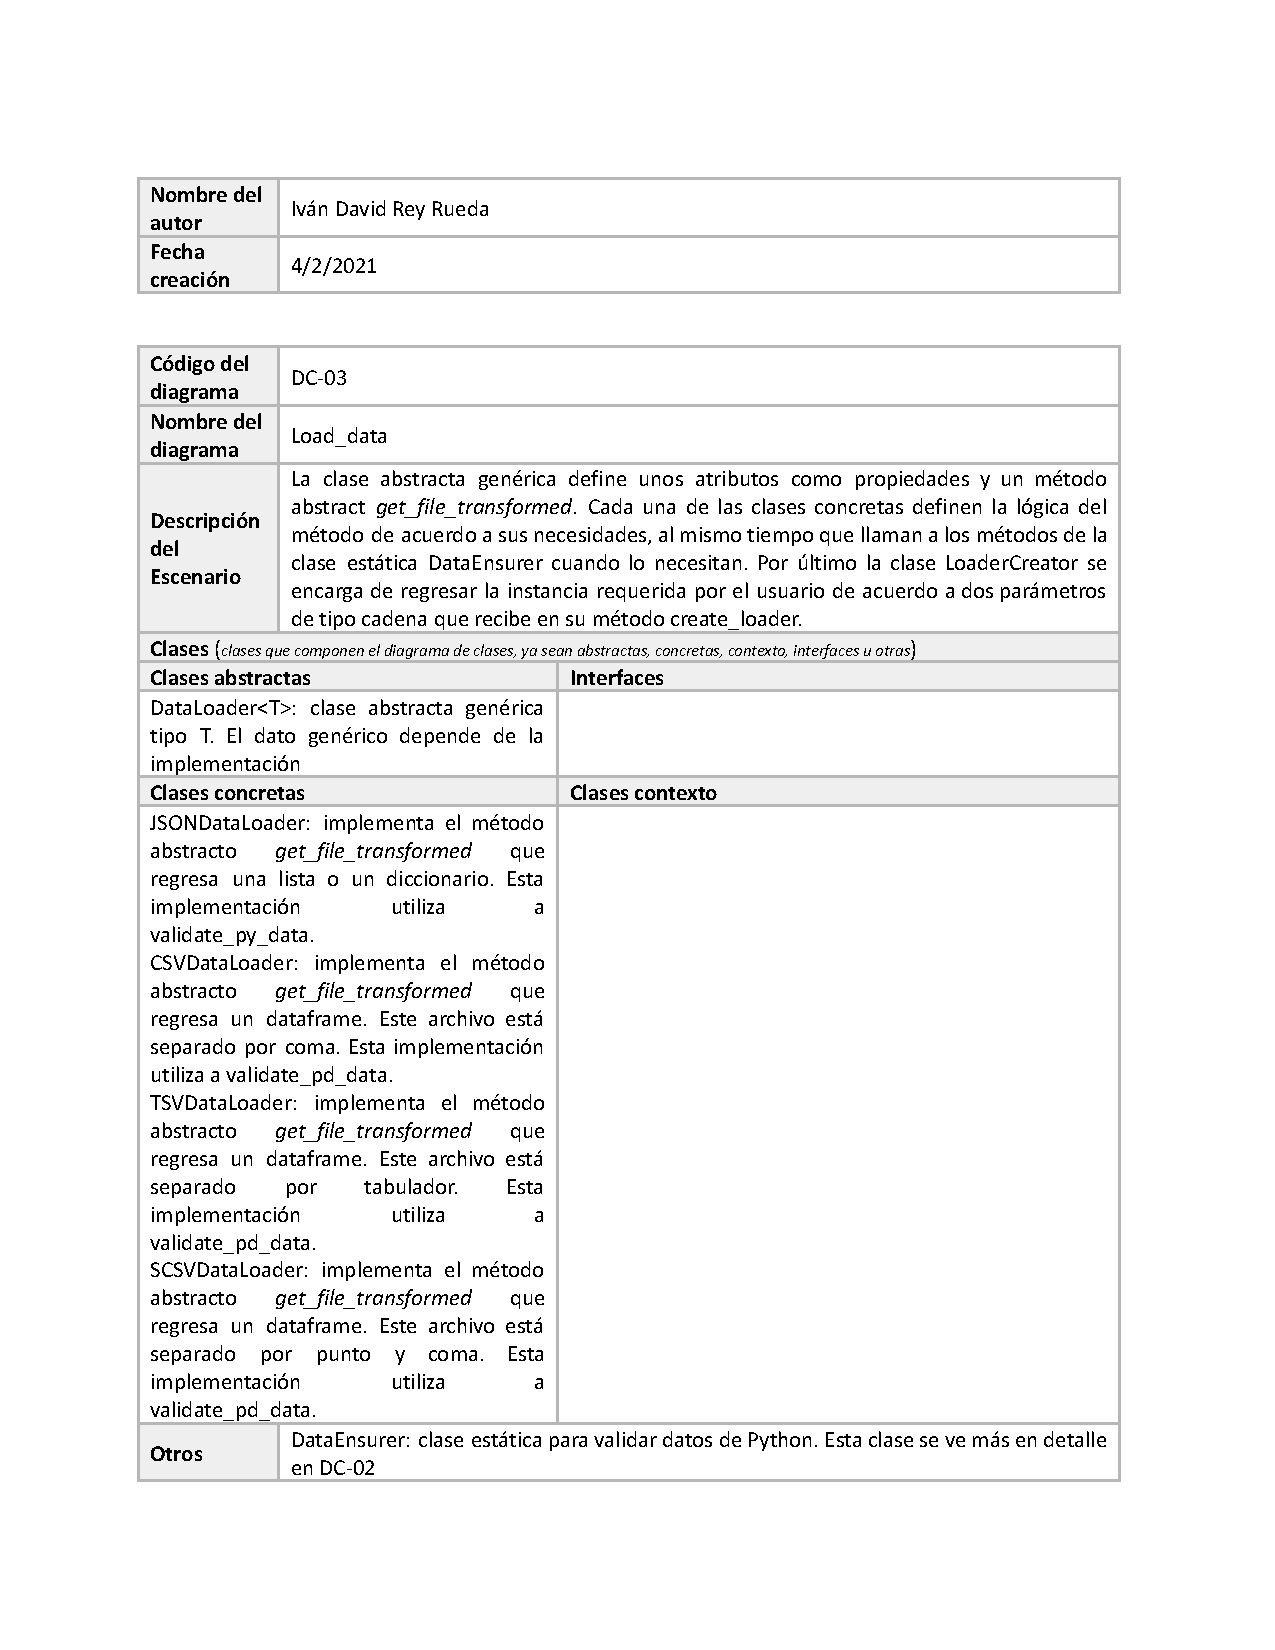
\includepdf[pages=-, pagecommand=\thispagestyle{otherplain}, width=\textwidth]{pdfs/Formato diagrama de clase DC-03_Firmado.pdf}
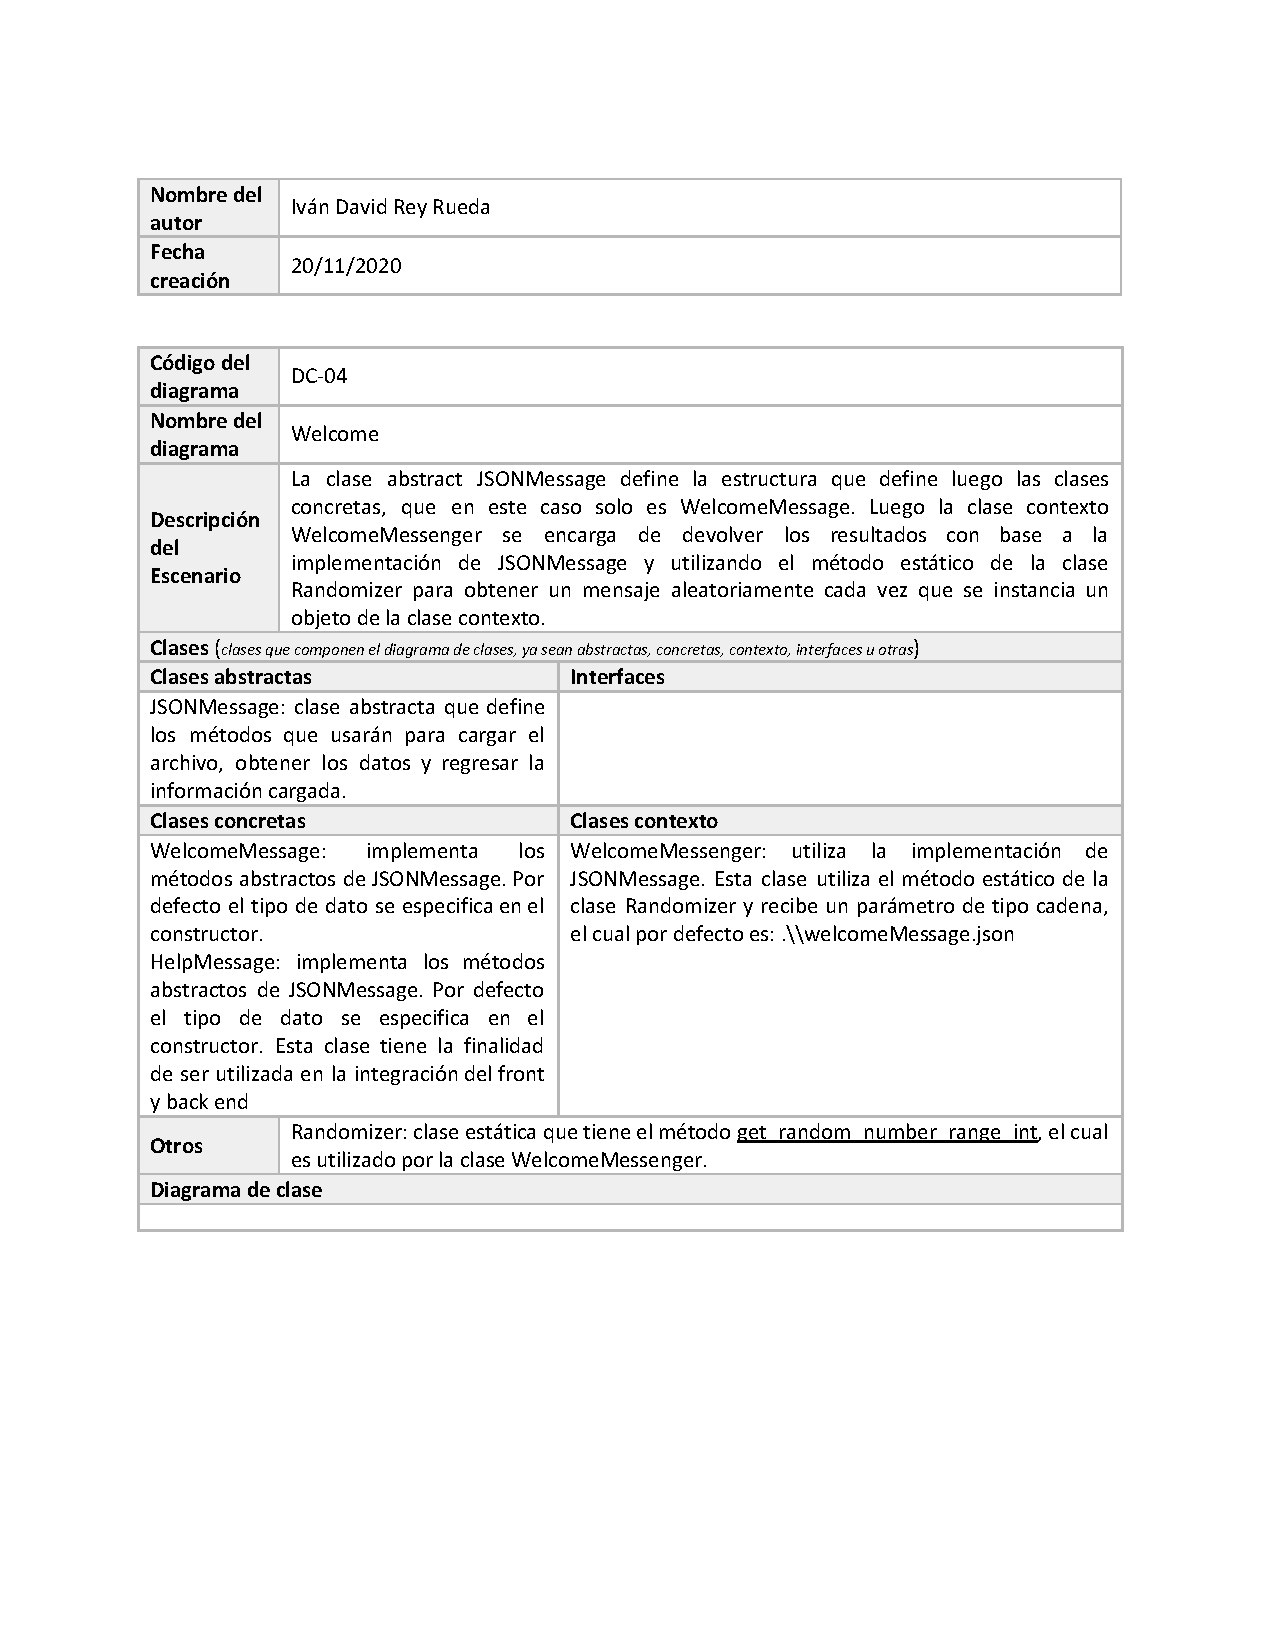
\includepdf[pages=-, pagecommand=\thispagestyle{otherplain}, width=\textwidth]{pdfs/Formato diagrama de clase DC-04_Firmado.pdf}
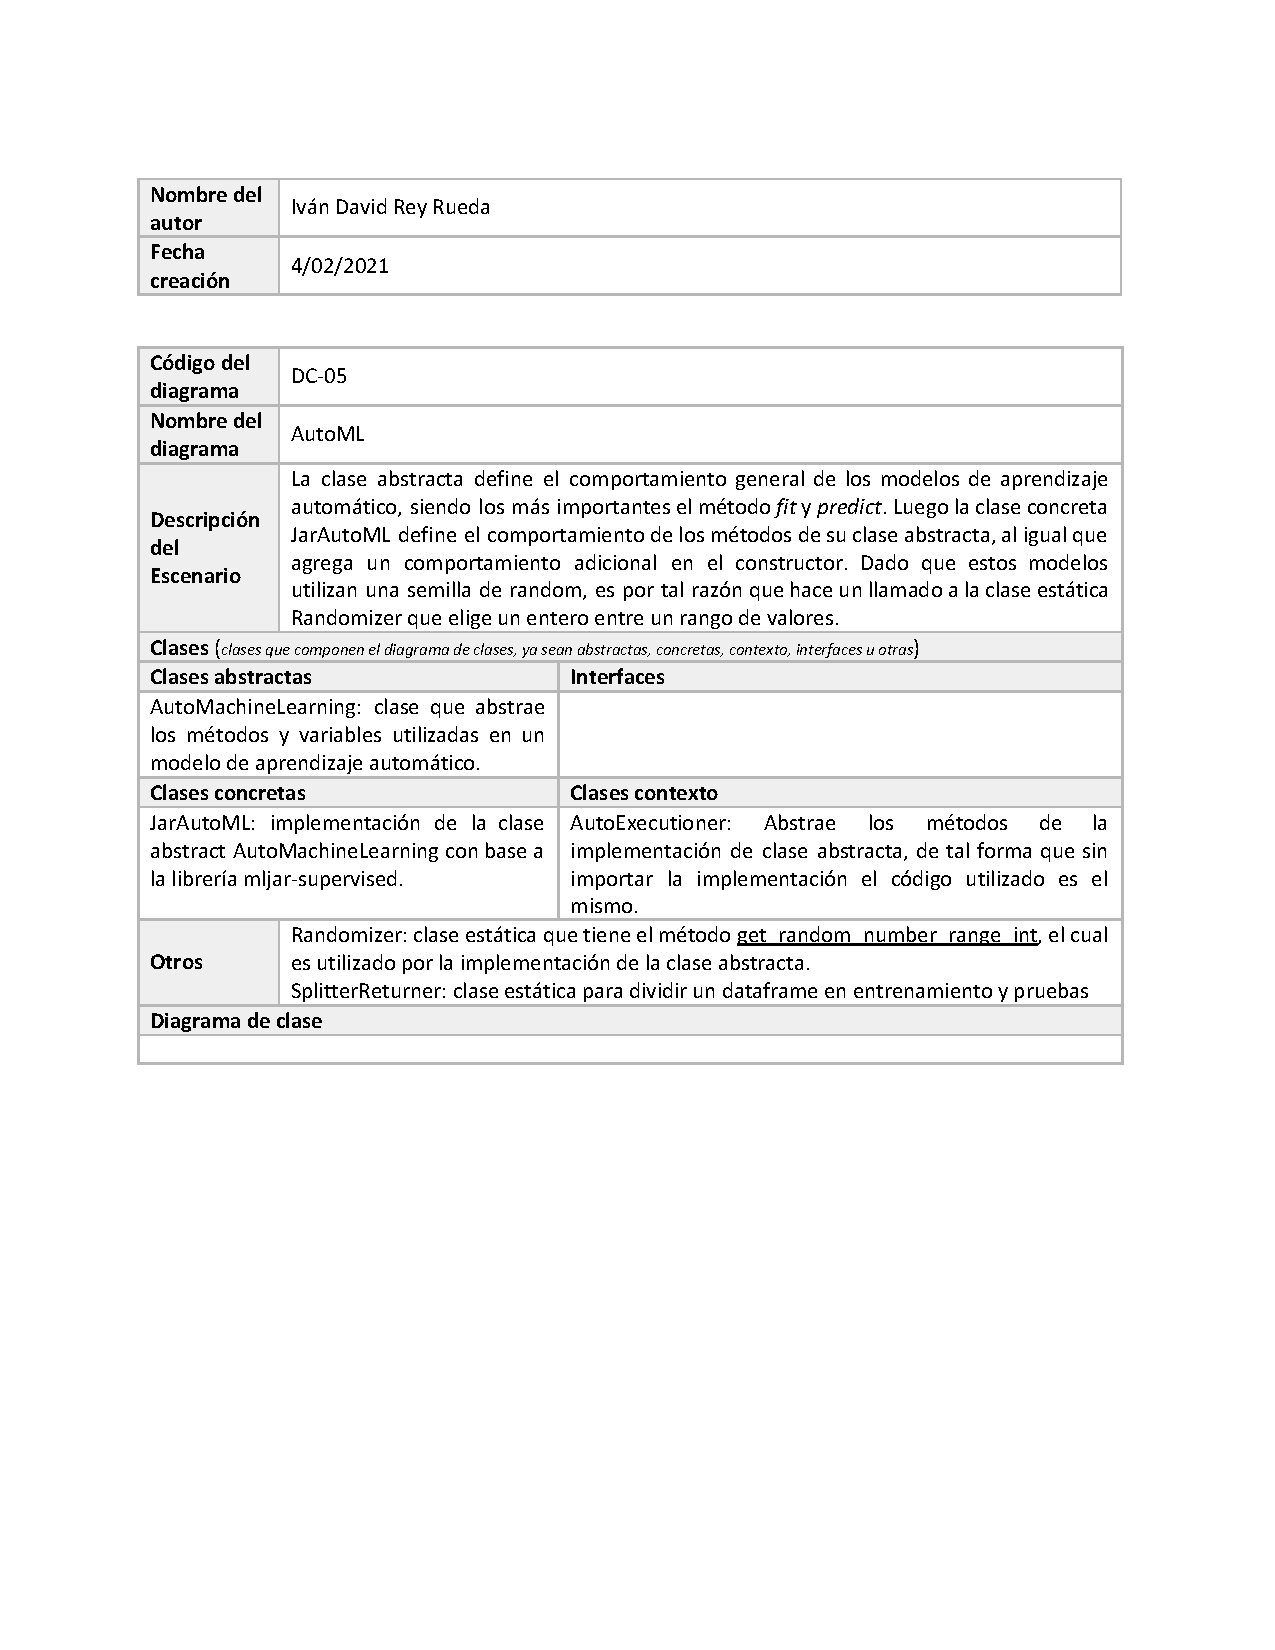
\includepdf[pages=-,pagecommand=\thispagestyle{otherplain}, width=\textwidth]{pdfs/Formato diagrama de clase DC-05_Firmado.pdf}
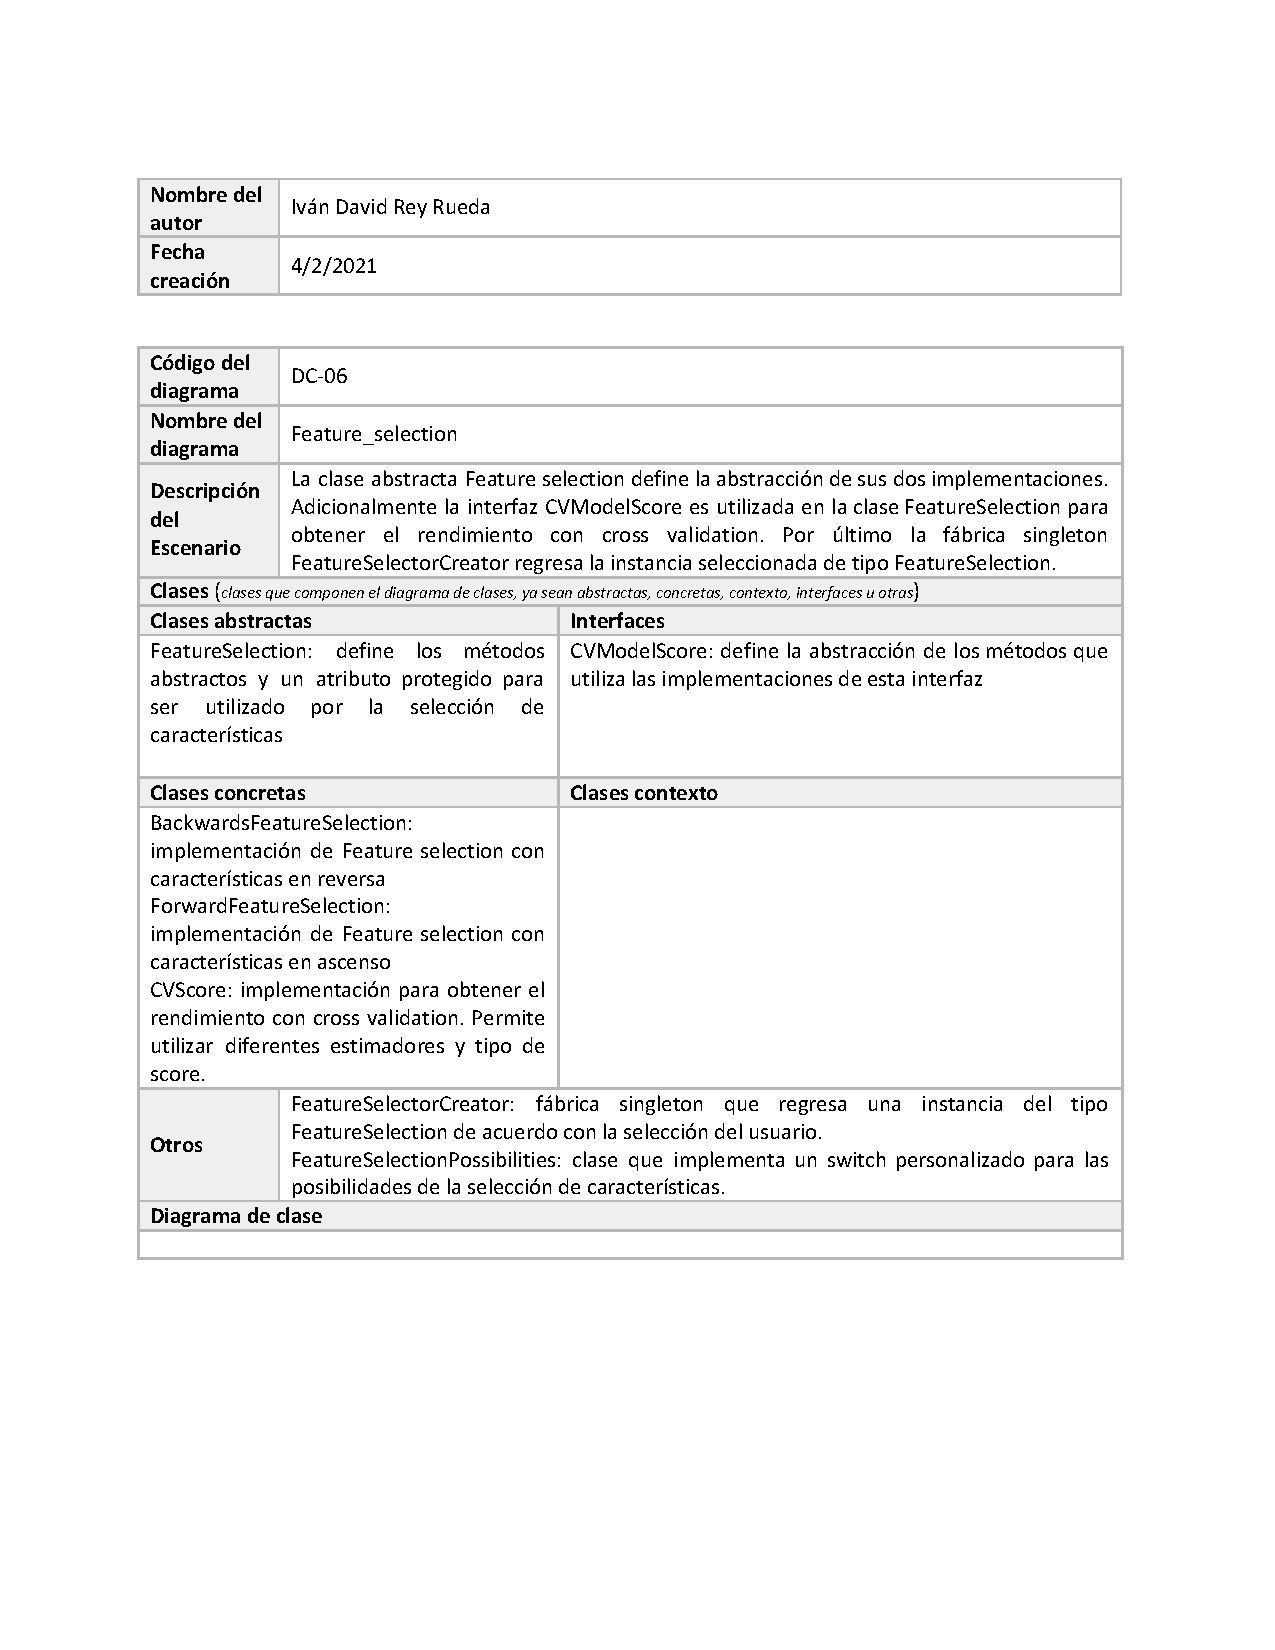
\includepdf[pages=-, pagecommand=\thispagestyle{otherplain}, width=\textwidth]{pdfs/Formato diagrama de clase DC-06_Firmado.pdf}
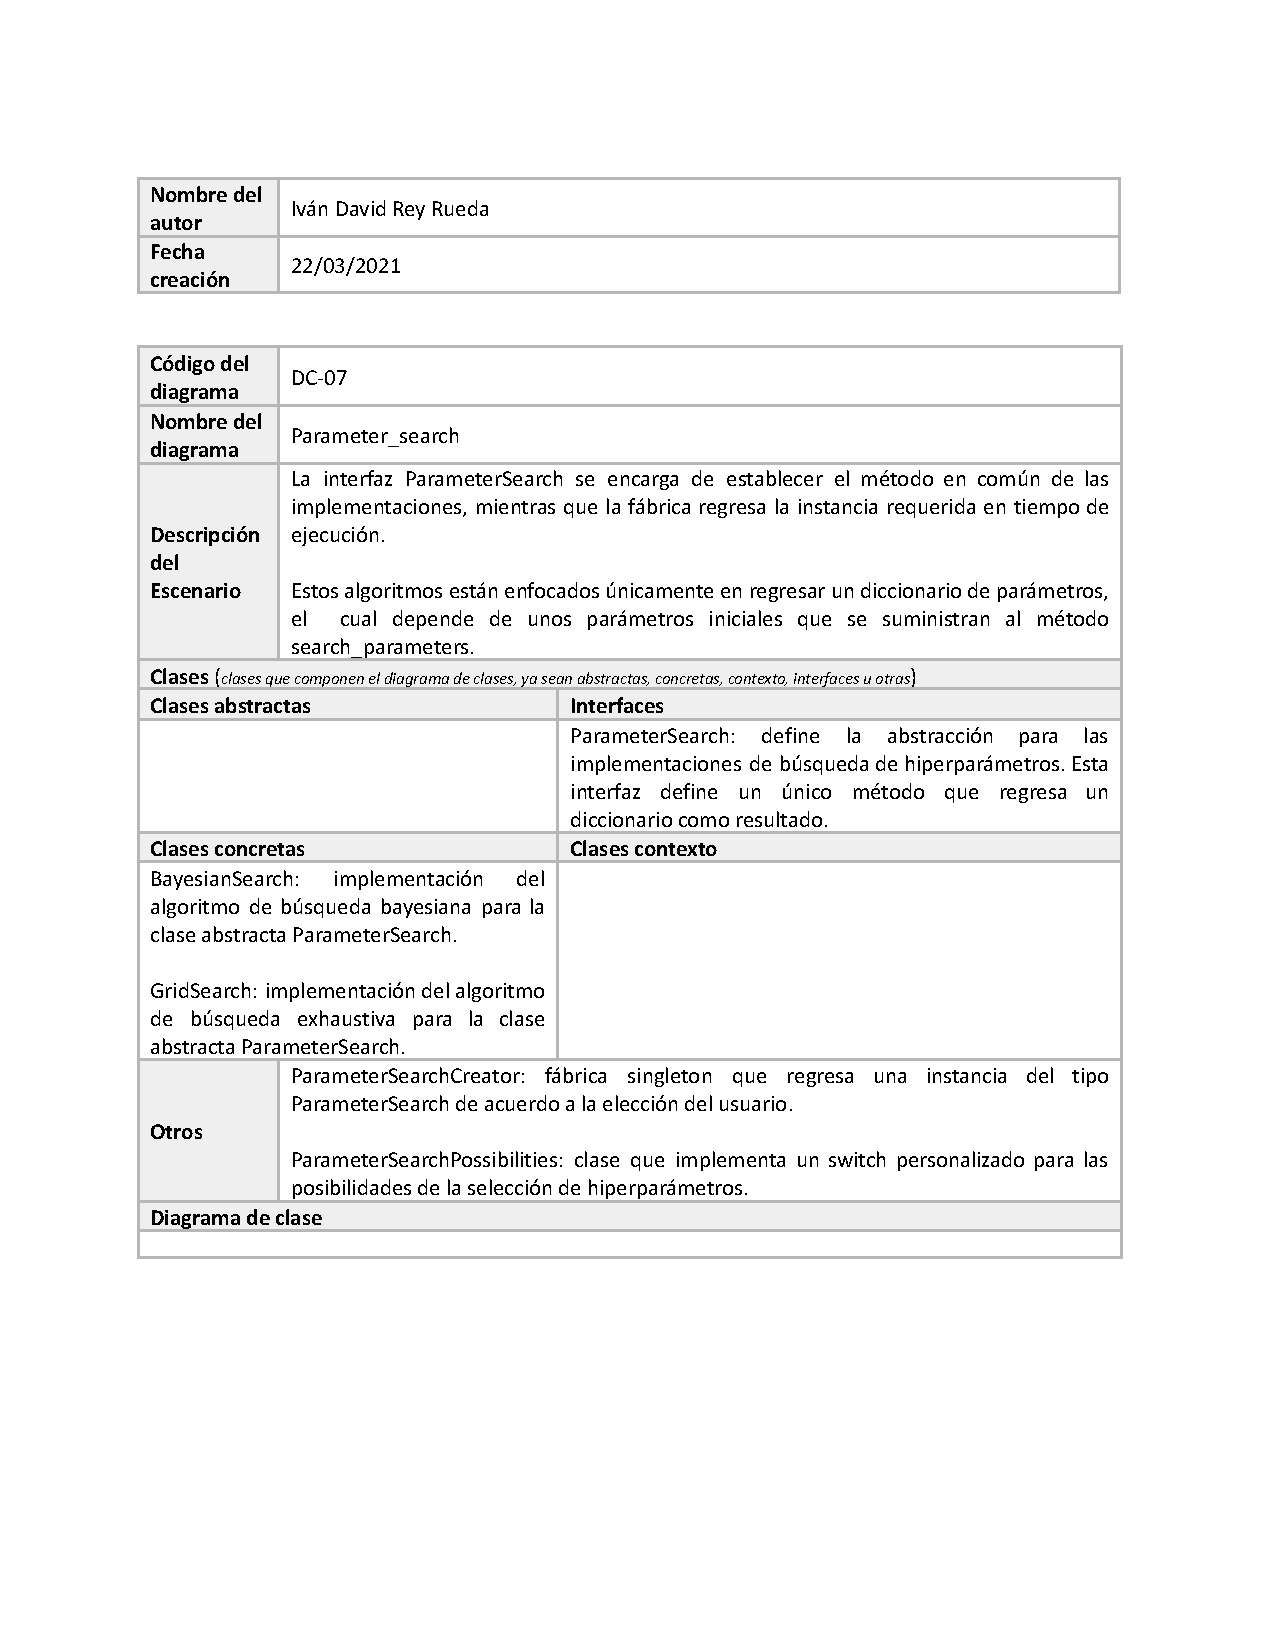
\includepdf[pages=-, pagecommand=\thispagestyle{otherplain}, width=\textwidth]{pdfs/Formato diagrama de clase DC-07_Firmado.pdf}
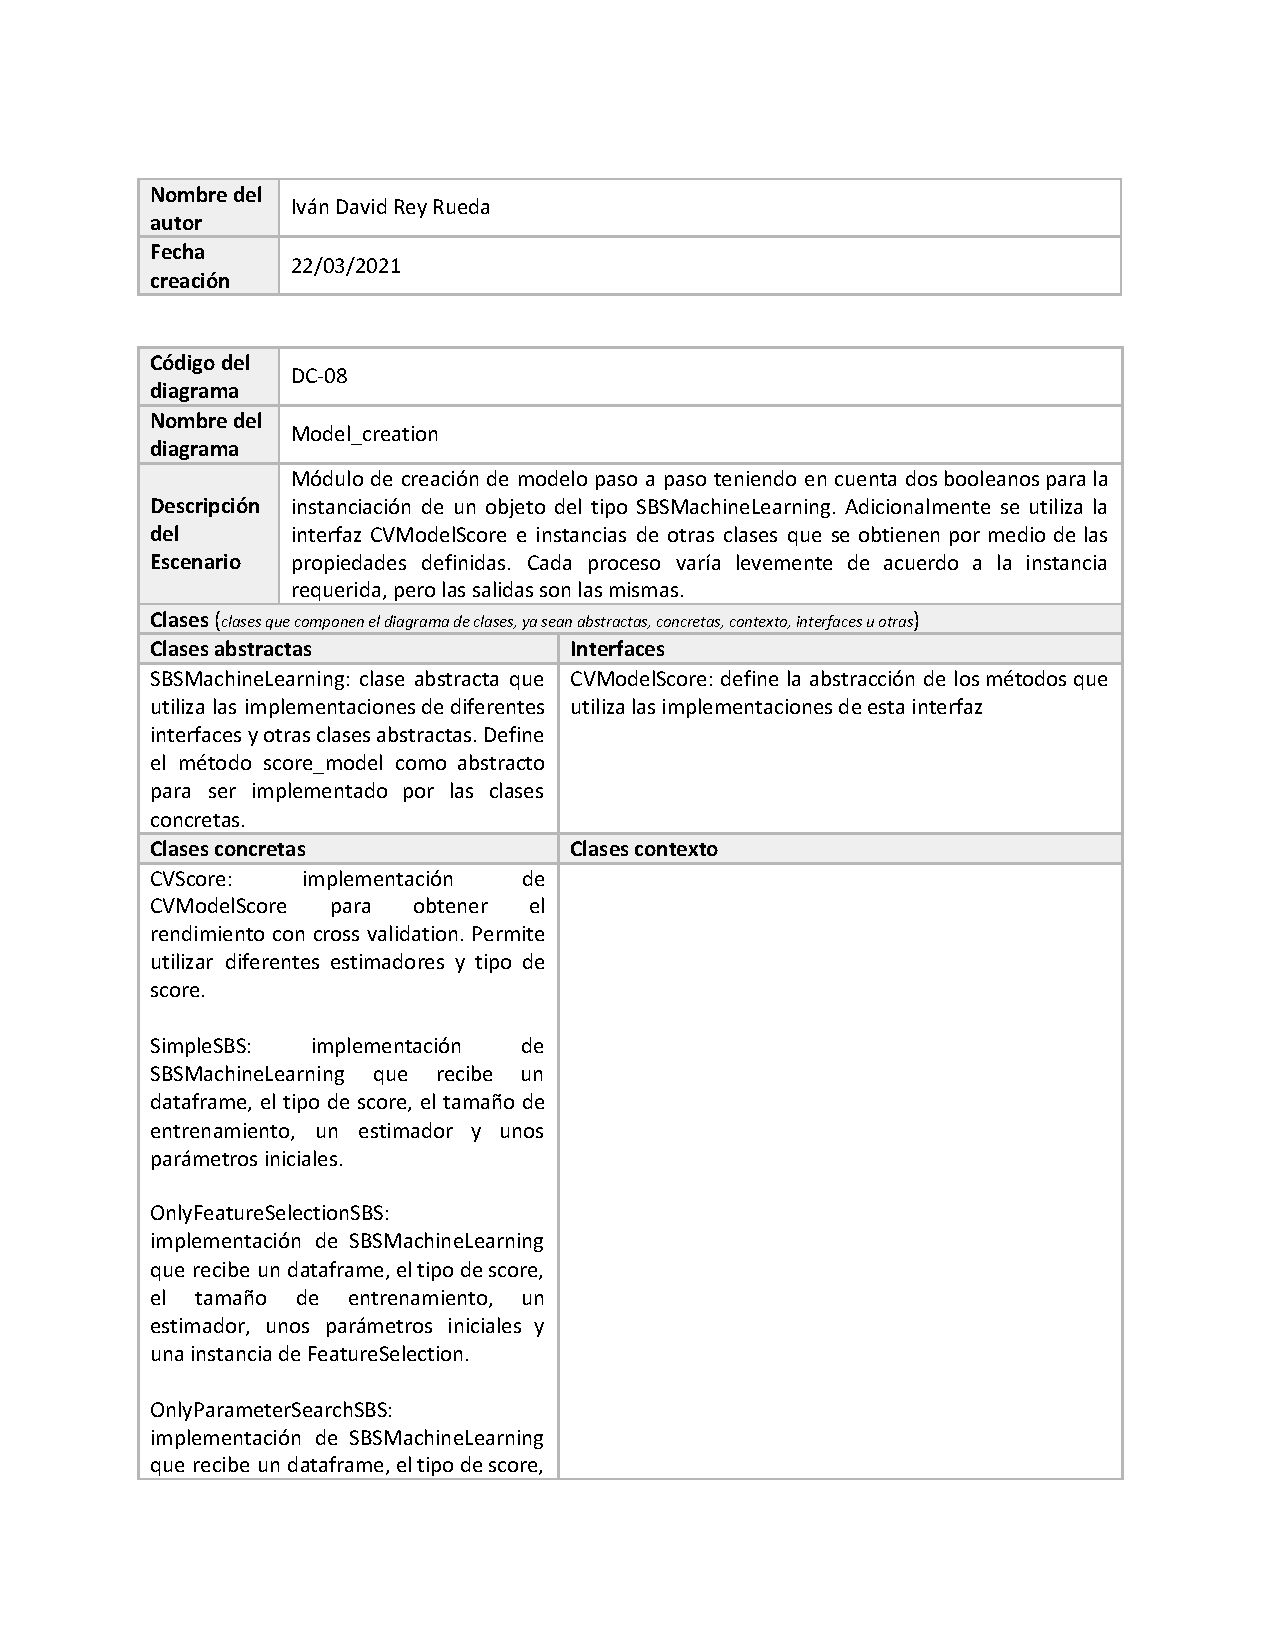
\includepdf[pages=-, pagecommand=\thispagestyle{otherplain}, width=\textwidth]{pdfs/Formato diagrama de clase DC-08_Firmado.pdf}
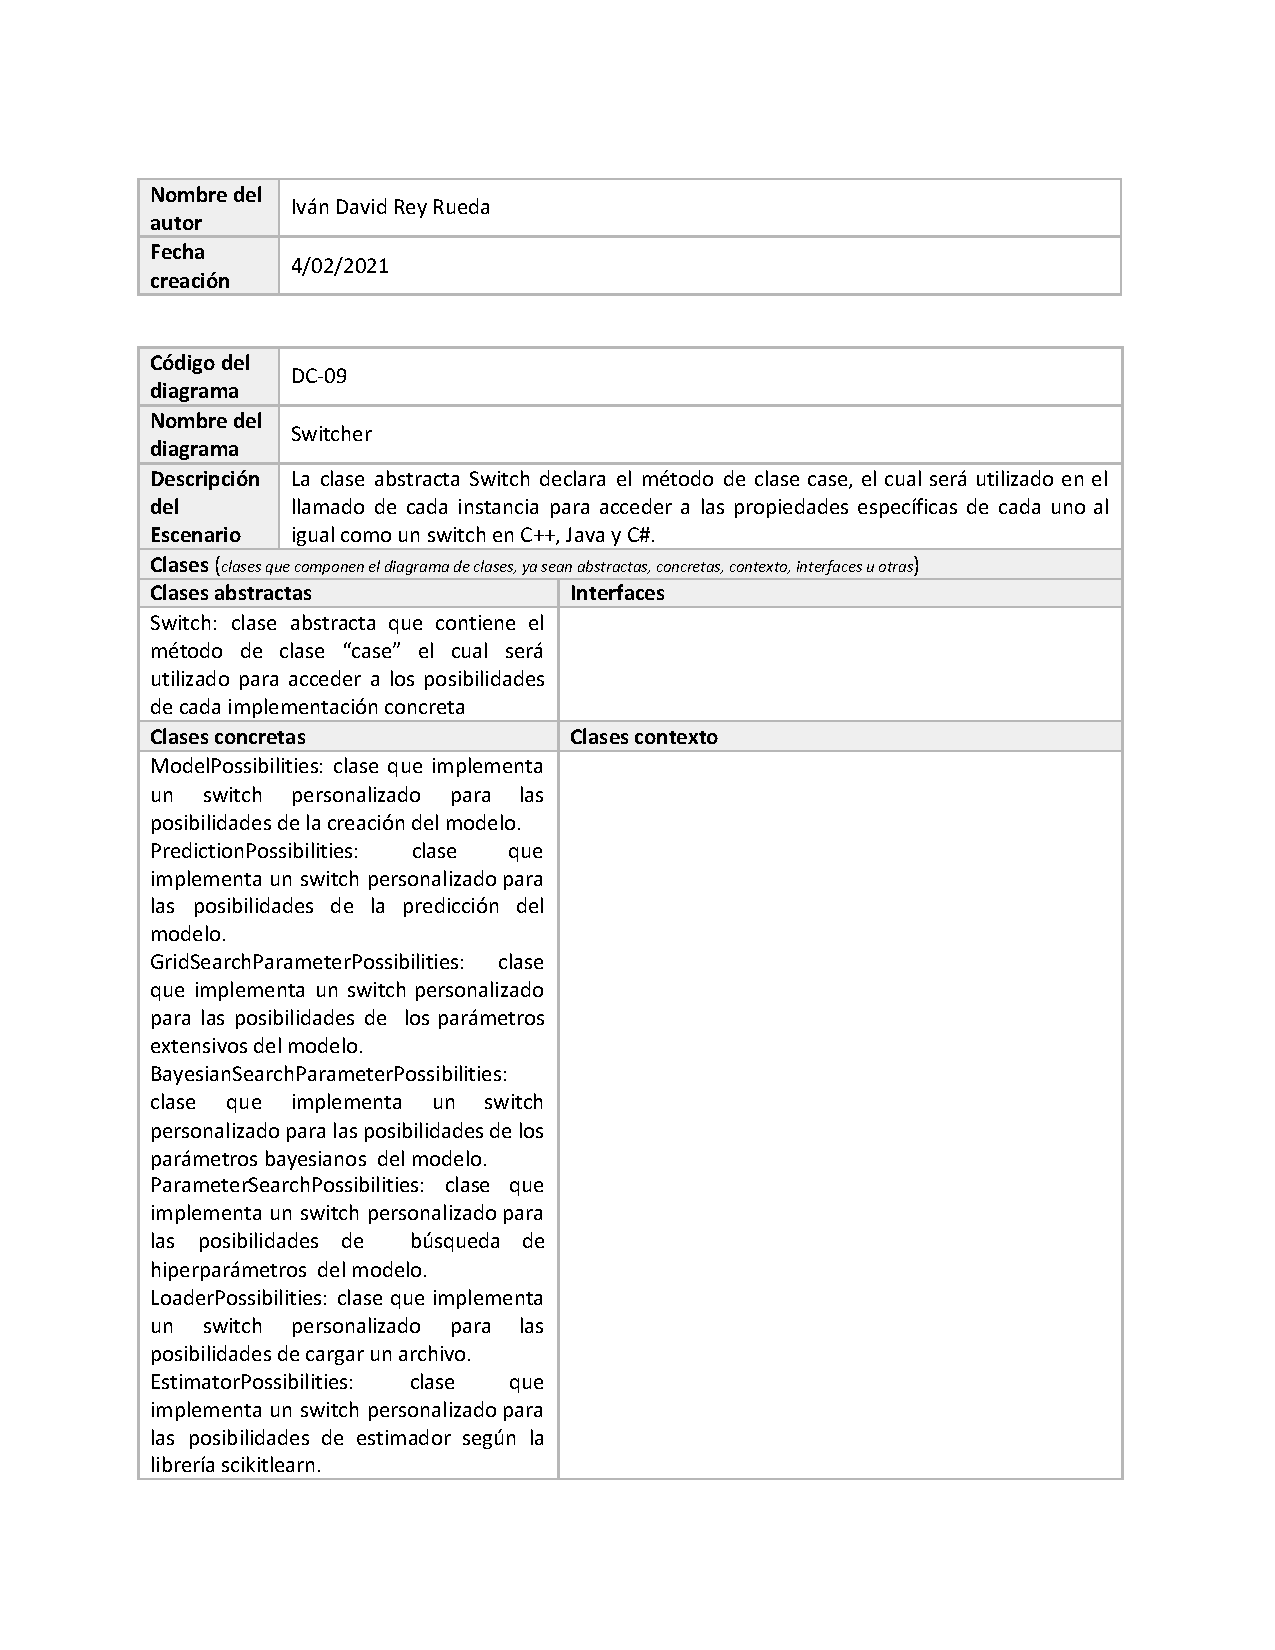
\includepdf[pages=-, pagecommand=\thispagestyle{otherplain}, width=\textwidth]{pdfs/Formato diagrama de clase DC-09_Firmado.pdf}
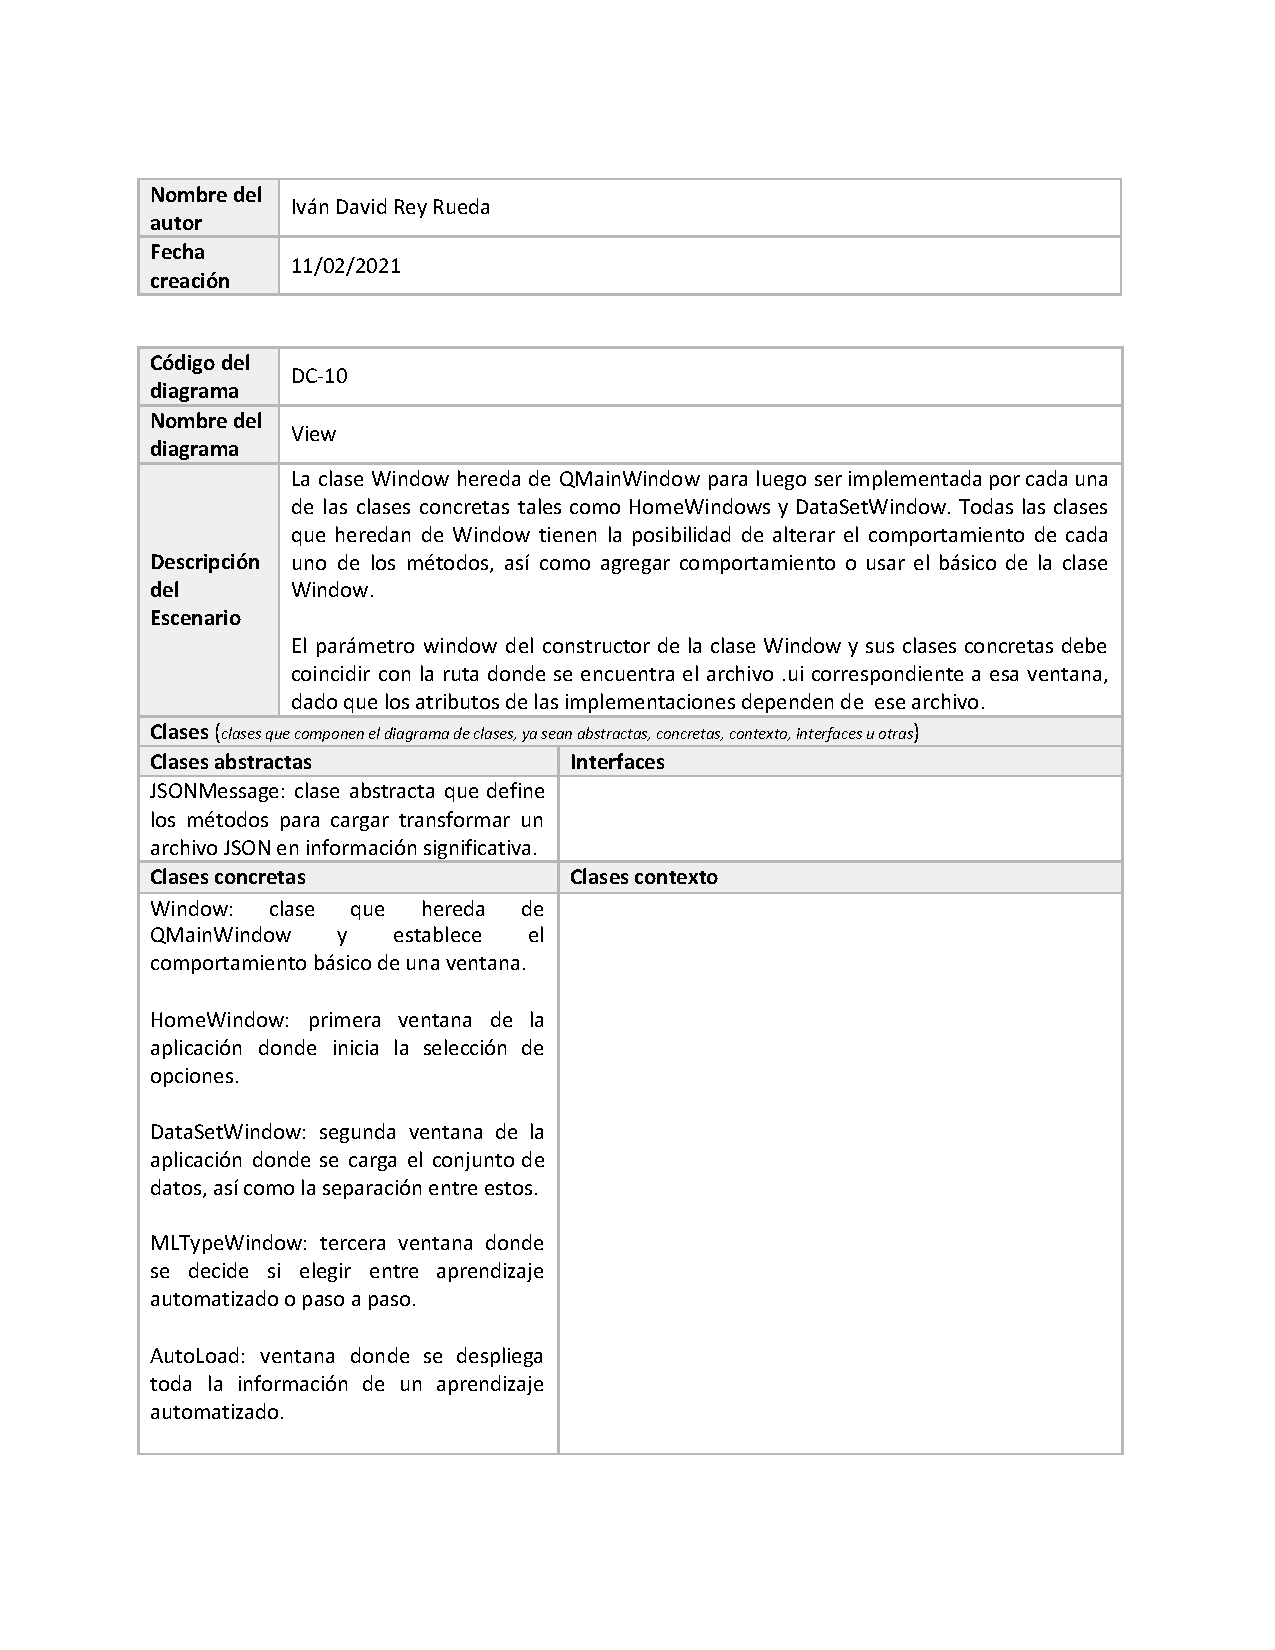
\includepdf[pages=-, pagecommand=\thispagestyle{otherplain}, width=\textwidth]{pdfs/Formato diagrama de clase DC-10_Firmado.pdf}
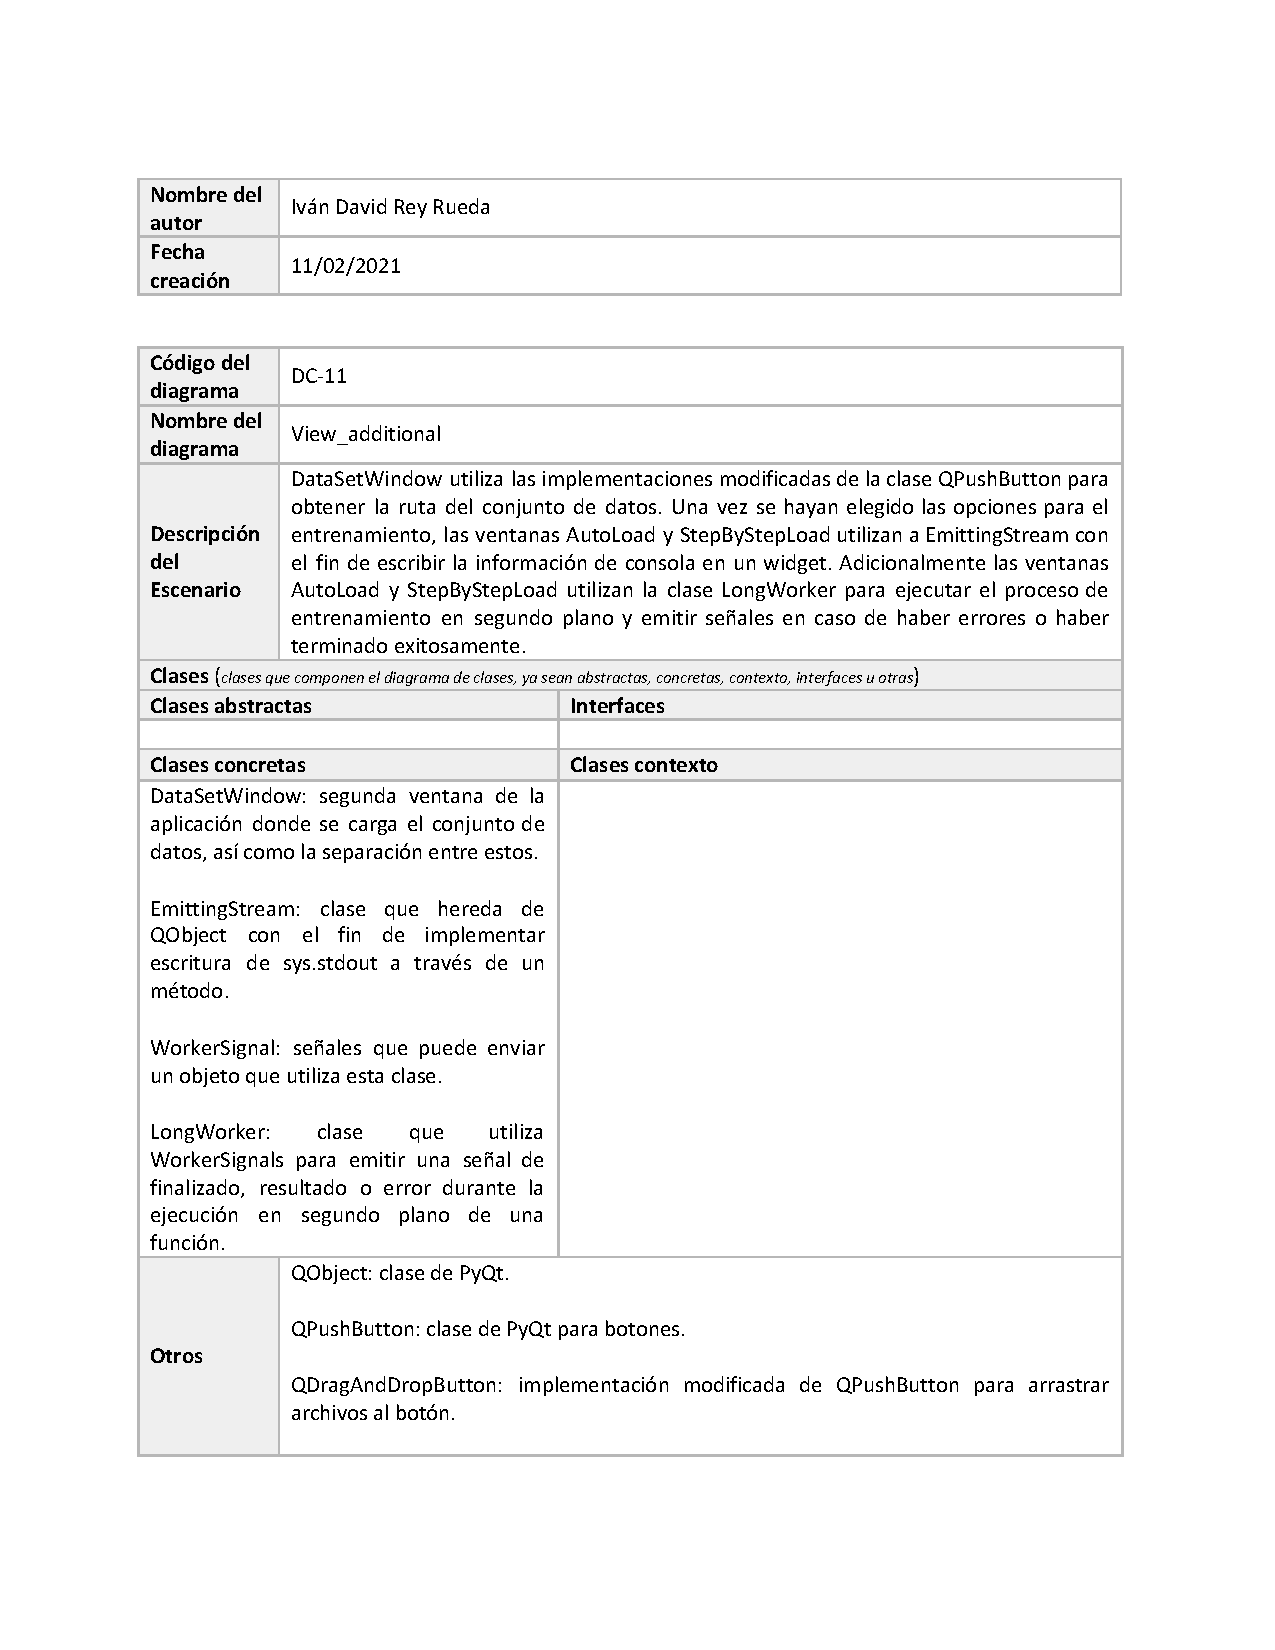
\includepdf[pages=-, pagecommand=\thispagestyle{otherplain}, width=\textwidth]{pdfs/Formato diagrama de clase DC-11_Firmado.pdf}

% casos de uso

% pruebas de software